%% multiple_genome_alignment.tex
%% Author: Leighton Pritchard
%% Copyright: James Hutton Institute
%% Multiple genome alignment approaches

%
\begin{frame}
  \frametitle{Multiple genome alignments}
  \textcolor{olive}{Multiple genome alignments are ``harder'' than pairwise} \\
  \begin{itemize}
    \item Computationally difficult to produce
    \item \textcolor{red}{Lead to NP-complete optimisation problems!}
  \end{itemize}  
  \textcolor{hutton_green}{Solutions:} \textbf{heuristics}
  \begin{itemize}
    \item Progressive (build a tree, combine pairwise alignments)
    \item Iterative (realign initial sequences as new genomes added)
    \item \textcolor{hutton_blue}{Positional homology}
    \item \textcolor{hutton_purple}{\textit{Glocal} alignments}
  \end{itemize}  
\end{frame}

%
\begin{frame}
  \frametitle{Multiple genome alignment}
  Many tools either positional homology or glocal alignment
  \begin{columns}[T] 
    \column{.5\textwidth} 
      \textcolor{olive}{Several tools:}
      \begin{itemize}
        \item Mugsy: {\tiny\href{http://mugsy.sourceforge.net/}{(http://mugsy.sourceforge.net/)}}
        \item \textcolor{hutton_blue}{MLAGAN: {\tiny\href{http://lagan.stanford.edu/lagan_web/index.shtml}{(http://lagan.stanford.edu/lagan\_web/index.shtml)}}}
        \item TBA/MultiZ: {\tiny\href{http://www.bx.psu.edu/miller_lab/}{(http://www.bx.psu.edu/miller\_lab/)}}
        \item \textcolor{red}{\textbf{Mauve}: {\tiny\href{http://gel.ahabs.wisc.edu/mauve/}{(http://gel.ahabs.wisc.edu/mauve/)}}}
      \end{itemize}
    \column{.5\textwidth}
      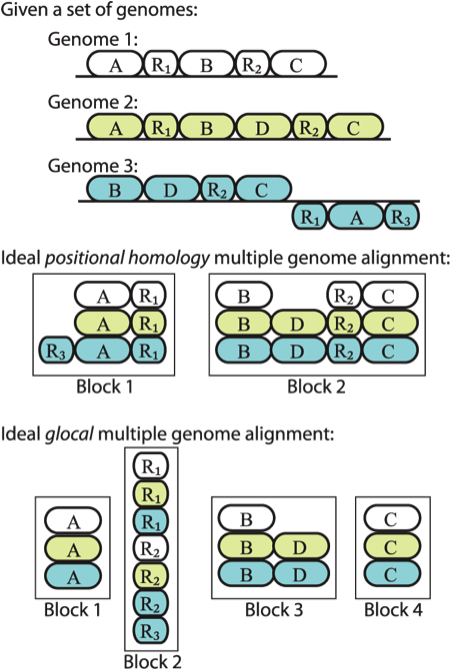
\includegraphics[width=0.75\textwidth]{images/poshom_v_glocal}
  \end{columns}    
\end{frame}

%
\begin{frame}
  \frametitle{LAGAN
  \footnote{\tiny{\href{http://dx.doi.org/10.1101/gr.926603
}{Brudno \textit{et al.} (2003) \textit{Genome Res.} doi:10.1101/gr.926603
}}}
  }
  Rapid pairwise alignment of homologous genomes
  \begin{columns}[T] 
    \column{.55\textwidth} 
      \textcolor{olive}{Algorithm:}
      \begin{enumerate}
        \item \textcolor{hutton_green}{Generate local alignments {\small(\textit{anchors}, B)}}
        \item \textcolor{hutton_blue}{Construct rough global map {\small(\textit{max-scoring ordered subset}, C)}}
        \item Join anchors that lie within a threshold distance
        \item \textcolor{hutton_purple}{Compute global alignment within each anchor {\small(\textit{Needleman-Wunsch}, D)}}
      \end{enumerate}
    \column{.45\textwidth}
      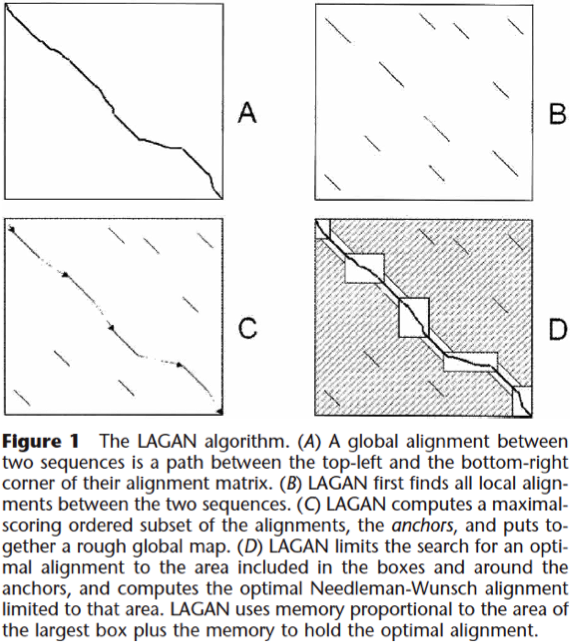
\includegraphics[width=\textwidth]{images/lagan_method}
  \end{columns}    
\end{frame}

%
\begin{frame}
  \frametitle{MLAGAN
  \footnote{\tiny{\href{http://dx.doi.org/10.1101/gr.926603
}{Brudno \textit{et al.} (2003) \textit{Genome Res.} doi:10.1101/gr.926603
}}}
  }
  Multiple genome alignment of $k$ genomes in $k-1$ alignment steps \\
  Progressive/iterative, using phylogenetic tree (like \texttt{CLUSTAL})
  \begin{columns}[T] 
    \column{.55\textwidth} 
      \textcolor{olive}{Algorithm:}
      \begin{enumerate}
        \item \textcolor{hutton_green}{Construct rough global maps between each pair of sequences {\small(step C in LAGAN)}}
        \item \textcolor{hutton_blue}{Progressive multiple alignment with anchors:}
		\begin{itemize}
          \item \textcolor{hutton_purple}{LAGAN alignment between closest pair of sequences: combined as \textit{multi-sequences}}
          \item \textcolor{hutton_purple}{Find rough global maps of this multi-sequence to all other multi-sequences}          
        \end{itemize}
      \end{enumerate}
    \column{.45\textwidth}
      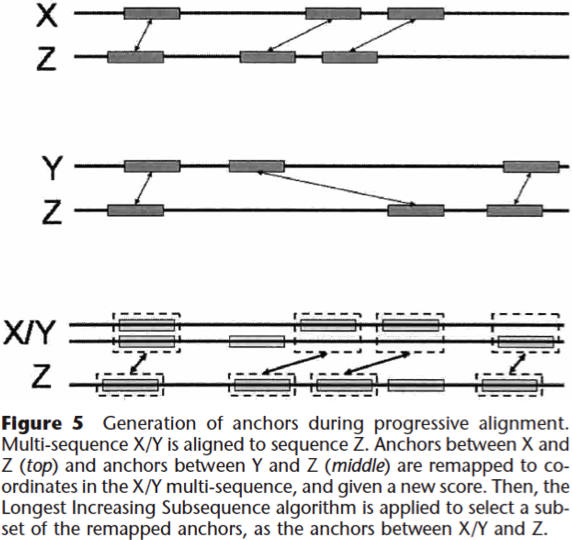
\includegraphics[width=\textwidth]{images/mlagan_method}
  \end{columns}    
\end{frame}

%
\begin{frame}
  \frametitle{Human:Mouse:Rat}
  \begin{center}
    
\includegraphics[height=0.7\textheight]{images/mouse-rat-photo}
  \end{center}
\end{frame}

%
\begin{frame}
  \frametitle{Human:Mouse:Rat
  \footnote{\tiny{\href{http://dx.doi.org/10.1101/gr.2067704
}{Brudno \textit{et al.} (2004) \textit{Genome Res.} doi:10.1101/gr.2067704
}}}
  }
  \textcolor{hutton_green}{Three-way progressive alignment} 
  \begin{columns}[T] 
    \column{.4\textwidth} 
    \textcolor{hutton_blue}{Initial alignments: BLAT \\
    Synteny: LAGAN/MLAGAN \\~\\}
    \textcolor{hutton_purple}{Three-way synteny}
      \begin{itemize}
        \item Homologous (HMR)
        \item Rodent-only (MR)
        \item Human-mouse (HM)
        \item Human-rat (HR)
      \end{itemize}
    \column{.6\textwidth}
      \begin{center}
        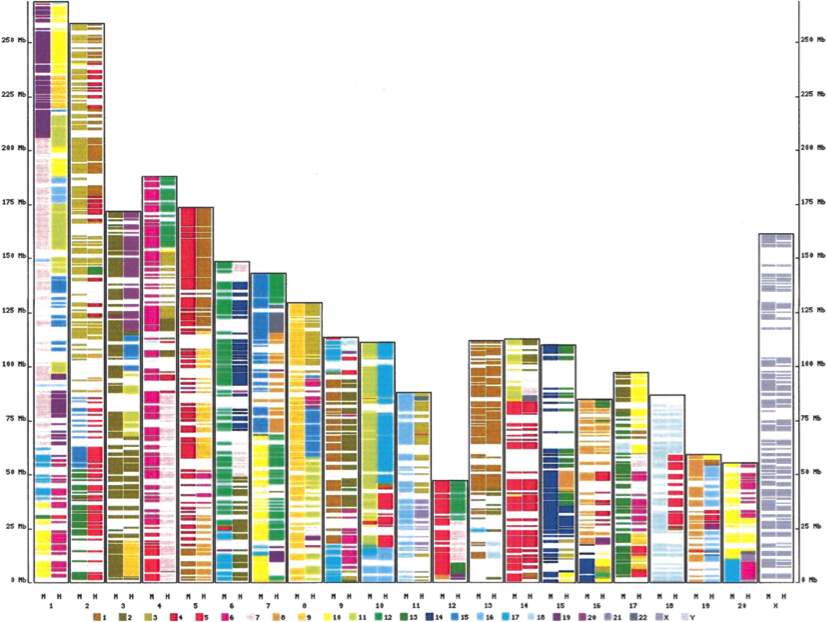
\includegraphics[width=\textwidth]{images/hmr_alignment} \\
        {\tiny(synteny mapped to rat genome)}
      \end{center}
  \end{columns}    
\end{frame}